pdfoutput=1
\pdfoutput=1
% ========================================================================
% SCX Internal Document
% Beyond Metaphor: Quantum Entanglement, Data WormholesRelativistic InvarianceSCX
% Beyond Metaphor: Rigorous Formalization of Quantum Entanglement,
% Data Wormholes, and Relativistic Invariance in SCX Auditing
%
% Author: Xiaogan Supercomputing Center (SCX)
% Classification: INTERNAL
% Date: 2026-07-02
% Lines: 1000+
% Source: entanglement_wormhole_relativity.md (Rounds 1--2)
% entanglement_rounds_3_5.md (Rounds 3--5, FORMALIZED)
% ========================================================================
\documentclass[11pt,a4paper]{article}
% --- Packages ---
\usepackage[T1]{fontenc}
\usepackage{amsmath,amssymb,amsfonts}
\usepackage{mathtools}
\usepackage{bm}
\usepackage{graphicx}
\usepackage{hyperref}
\usepackage{xcolor}
\usepackage{tikz}
\usepackage{tikz-cd}
\usepackage{enumitem}
\usepackage{booktabs}
\usepackage{geometry}
\usepackage{fancyhdr}
\usepackage{titling}
\usepackage{abstract}
\usepackage{mathrsfs}
\usepackage{extarrows}
\usepackage{listings}
\usepackage{tcolorbox}
\usepackage{amsthm}
\usepackage{algorithm}
\usepackage{algpseudocode}
\geometry{margin=2.5cm}
% --- Chinese support ---
% --- Custom colors ---
\definecolor{scxblue}{RGB}{0,51,102}
\definecolor{scxgold}{RGB}{204,153,0}
\definecolor{darkred}{RGB}{139,0,0}
\definecolor{darkgreen}{RGB}{0,100,0}
\definecolor{verdictgreen}{RGB}{34,139,34}
\definecolor{verdictyellow}{RGB}{204,153,0}
\definecolor{verdictblue}{RGB}{0,102,204}
% --- Hyperref setup ---
\hypersetup{
 colorlinks=true,
 urlcolor=scxblue,
 citecolor=darkgreen
% --- Theorem environments ---
\theoremstyle{plain}
\newtheorem{theorem}{Theorem}[section]
\newtheorem{lemma}[theorem]{Lemma}
\newtheorem{proposition}[theorem]{Proposition}
\newtheorem{corollary}[theorem]{Corollary}
\theoremstyle{definition}
\newtheorem{definition}[theorem]{Definition}
\newtheorem{example}[theorem]{Example}
\theoremstyle{remark}
\newtheorem{remark}[theorem]{Remark}
% --- Custom commands ---
\newcommand{\RR}{\mathbb{R}}
\newcommand{\CC}{\mathbb{C}}
\newcommand{\ZZ}{\mathbb{Z}}
\newcommand{\NN}{\mathbb{N}}
\newcommand{\EE}{\mathbb{E}}
\newcommand{\PP}{\mathbb{P}}
\newcommand{\cM}{\mathcal{M}}
\newcommand{\cX}{\mathcal{X}}
\newcommand{\cC}{\mathcal{C}}
\newcommand{\cG}{\mathcal{G}}
\newcommand{\cI}{\mathcal{I}}
\newcommand{\cF}{\mathcal{F}}
\newcommand{\cH}{\mathcal{H}}
\DeclareMathOperator{\Cercis}{Cercis}
\DeclareMathOperator{\Var}{Var}
\DeclareMathOperator{\Cov}{Cov}
\DeclareMathOperator{\MMD}{MMD}
\DeclareMathOperator{\vol}{vol}
\DeclareMathOperator{\diam}{diam}
\DeclareMathOperator{\SAR}{SAR}
\DeclareMathOperator{\Stab}{Stab}
\DeclareMathOperator{\Diff}{Diff}
\DeclareMathOperator{\Isom}{Isom}
% --- Title box ---
\newtcolorbox{scxbox}[1][]{
 colback=scxblue!5,
 colframe=scxblue,
 fonttitle=\bfseries,
 title=#1
\newtcolorbox{verdictbox}[1][]{
 colback=#1!10,
 colframe=#1!60,
 fonttitle=\bfseries,
 title= / Verdict
% --- Bilingual block ---
\newenvironment{bilingual}[1]{%
 \medskip\noindent\textbf{#1}\par\nobreak
}{%
 \medskip
% ========================================================================
\begin{document}
% ========================================================================
% TITLE PAGE
% ========================================================================
\title{
 \vspace{2cm}
 {\Huge \textbf{Beyond Metaphor}}\\[0.2cm]
 {\LARGE Quantum Entanglement, Data WormholesRelativistic InvarianceSCX}\\[0.5cm]
 {\large \textcolor{scxblue}{Beyond Metaphor: Rigorous Formalization of}}\\[0.1cm]
 {\large \textcolor{scxblue}{Quantum Entanglement, Data Wormholes, and}}\\[0.1cm]
 {\large \textcolor{scxblue}{Relativistic Invariance in SCX Auditing}}\\[1cm]
 \rule{\textwidth}{1.5pt}\\[0.5cm]
 {\normalsize Xiaogan Supercomputing Center (SCX)}\\[0.2cm]
 {\small \texttt{papers/scx\_acad\_mdta\_ilh/main.tex}}\\[0.2cm]
 {\small Classification: INTERNAL}\\[0.2cm]
 {\small Version 1.0 --- 2026-07-02}
 \vspace{1cm}
\author{SCX}
\date{}
\maketitle
\thispagestyle{empty}
% ========================================================================
% ABSTRACT
% ========================================================================
\begin{abstract}
\noindent
\textbf{Abstract: } SCX---(ACAD), (MDTA), (ILH)---.Quantum Entanglement, (Einstein-Rosen), \"\".: ACAD/(5+1), MDTA(5), ILHSCX(9).: ACAD, MDTA, ILH.:,.
\bigskip
\noindent
\textbf{Abstract:} This paper presents a rigorous mathematical formalization of three physics-inspired exploration paths in SCX auditing: Audit Correlation Asymmetry Detection (ACAD), Manifold Density Topology Analysis (MDTA), and Invariance Layered Hierarchy (ILH). These paths originate from conceptual analogies with quantum entanglement, wormholes (Einstein-Rosen bridges), and special relativity respectively, and have undergone five rounds of ``inspiration $\rightarrow$ correction $\rightarrow$ formalization $\rightarrow$ hostile review $\rightarrow$ final verdict.'' This paper presents the corrected final frameworks: ACAD provides information-theoretic/statistical-security tampering detection (5 theorems + 1 corollary), MDTA provides persistent-homology-based manifold shortcut audit risk assessment (5 theorems), and ILH documents SCX invariance structure via group theory (9 theorems). Each framework carries an honest verdict: ACAD is \textbf{conditionally useful}, MDTA is \textbf{pragmatically useful}, and ILH has \textbf{documentation value}. This paper adheres to the honesty principle: physics analogies are not disguised as mathematical correspondences, and each framework's limitations and fractures are explicitly stated.
\bigskip
\noindent
\textbf{Keywords:} SCX auditing, entanglement, wormholes, relativity, gauge invariance, information-theoretic security, persistent homology, manifold learning, group theory, audit formalization
\end{abstract}
\newpage
% ========================================================================
% TABLE OF CONTENTS
% ========================================================================
\tableofcontents
\newpage
% ========================================================================
% SECTION 1: INTRODUCTION
% ========================================================================
\section{ / Introduction}
\label{sec:intro}
\subsection{ / Background and Motivation}
SCXCoreHodge($U(1)$- + $O(d)$)..---\textbf{Quantum Entanglement}, (Einstein-Rosen)(Lorentz)---: SCXHodgePerspective?
\textit{SCX's core mathematical foundation is discrete Hodge theory + gauge theory ($U(1)$-type translation gauge + $O(d)$ lattice gauge). These tools originate from QFT and particle physics. This paper explores three deeper physics concepts --- quantum entanglement, wormholes (Einstein-Rosen bridges), and special relativity (Lorentz invariance) --- and honestly asks: do they provide audit perspectives not yet covered by discrete Hodge theory?}
\begin{table}[h]
\centering
\begin{tabular}{p{4.5cm} p{7cm}}
\toprule
\textbf{ / Physics Concept} & \textbf{SCX / SCX Audit Analog} \\
\midrule
\textit{Quantum entanglement: non-local correlation, Bell inequality} & \textit{Non-separable correlation between auditors --- tamper once, detect globally} \\
\addlinespace
\textit{Wormholes: spacetime shortcuts, Einstein-Rosen bridges} & \textit{Low-density tunnels on the Situs manifold --- data ``backdoors''} \\
\addlinespace
\textit{Relativity: Lorentz transformations preserve spacetime interval} & \textit{Cercis Score as gauge invariant --- audit ``proper time''} \\
\bottomrule
\end{tabular}
\caption{Core / Core Intuition Mapping}
\label{tab:intuition}
\end{table}
\subsection{ / Five-Round Iteration History}
\begin{enumerate}[leftmargin=*]
 \item \textbf{1: } --- SCX
 \item \textbf{2: } ---, 
 \item \textbf{3: } --- (,, Proof)
 \item \textbf{4: } --- 
 \item \textbf{5: } ---, 
\end{enumerate}
\textit{This paper presents frameworks that have undergone five complete iterations: (1) Creative exploration --- building analogical mappings; (2) Self-review and correction --- identifying mathematical fractures; (3) Rigorous formalization --- establishing explicit mathematical frameworks; (4) Hostile review --- searching for fractures in formalizations; (5) Fixes and final verdict --- repairing repairable fractures, honestly positioning each path's value.}
\subsection{ / Overview of Three Corrected Paths}
\begin{table}[h]
\centering
\begin{tabular}{p{2cm} p{3.5cm} p{3.5cm} p{3cm}}
\toprule
 &  &  &  \\
\textit{Path} & \textit{Original Analogy} & \textit{Corrected Framework} & \textit{Final Verdict} \\
\midrule
ACAD & Quantum Entanglement $\rightarrow$ Bellawaiting & (+MMD) &  \\
\textit{ACAD} & \textit{Entanglement $\rightarrow$ Bell audit} & \textit{Audit Correlation Asymmetry Detection} & \textit{Conditionally Useful} \\
\addlinespace
MDTA & $\rightarrow$ Data Wormholes & (+) &  \\
\textit{MDTA} & \textit{Wormholes $\rightarrow$ data shortcuts} & \textit{Manifold Density Topology Analysis} & \textit{Pragmatically Useful} \\
\addlinespace
ILH & $\rightarrow$ Cercis= & (+Galileo) &  \\
\textit{ILH} & \textit{Relativity $\rightarrow$ Cercis=spacetime} & \textit{Invariance Layered Hierarchy} & \textit{Documentation Value} \\
\bottomrule
\end{tabular}
\caption{ / Overview of Three Corrected Paths}
\label{tab:overview}
\end{table}
\subsection{ / Honesty Principle}
\begin{enumerate}[leftmargin=*]
 \item \textbf{: }, 
 \item \textbf{: } 
 \item \textbf{: } ---,,, 
 \item \textbf{: }, 
\end{enumerate}
\textit{This paper adheres to the following honesty principles: (1) Analogies are not disguised as correspondences; (2) Fractures are transparently presented alongside theorems; (3) A tiered verdict system is used; (4) Practical audit value is the ultimate criterion.}
\newpage
% ========================================================================
% PART I: ACAD
% ========================================================================
\part{ / ACAD}
\label{part:acad}
\begin{scxbox}[ / Path Trajectory]
\begin{tabular}{p{3cm} p{11cm}}
\textbf{1} & ``Quantum Entanglement''``Bellawaiting'' --- \\
\textit{Round 1} & \textit{``Quantum entangled reference states'' and ``Bell audit inequality''} \\
\textbf{2} & : Bellawaiting, Hilbert \\
\textit{Round 2} & \textit{Fractures: Bell inequality always holds classically, entanglement needs Hilbert space} \\
\textbf{3} & ACAD: \\
\textit{Round 3} & \textit{Formalized as ACAD: information-theoretic security tampering detection} \\
\textbf{4} & :, \\
\textit{Round 4} & \textit{Hostile review: security claims overstated, constraint construction incomplete} \\
\textbf{5} & : Serflingawaiting,, \\
\textit{Round 5} & \textit{Fixes: Serfling inequality, downgraded to statistical security, hash-chain constraints} \\
\end{tabular}
\end{scxbox}
\section{ACAD / ACAD Foundations}
\label{sec:acad-found}
\subsection{Core / Core Problem}
\begin{bilingual}{Core / Core Question}
$A$$B$,, ?
\textit{If two auditors $A$ and $B$ have reference data linked by a secret constraint, can tampering with one side be detected with high probability by an attacker ignorant of the constraint?}
\end{bilingual}
---(QKD).ACAD:.
\textit{This is an information-theoretic security problem --- sharing intuition with QKD but not its mathematics. ACAD corrects the entanglement analogy into an honest information-theoretic framework requiring no quantum mechanics.}
\subsection{ / Basic Definitions}
\begin{definition}[ / Audit Pair]
\label{def:audit-pair}
$(\cA, \cB, \cC)$, : 
\begin{itemize}
 \item $\cA \subseteq \cX^n$: $A$($n$)
 \item $\cB \subseteq \cX^n$: $B$
 \item $\cC \subseteq \{C: \cX \times \cX \to \{0,1\}\}$: 
\end{itemize}
\end{definition}
\begin{definition}[ / Secret Pairing]
\label{def:secret-pairing}
$\phi: [n] \to [n]$$C \in \cC$, : 
\begin{itemize}
 \item $A$$\{x_i^A\}_{i=1}^n$$\phi$$\{x_j^B\}_{j=1}^n$
 \item $B$$\{x_j^B\}_{j=1}^n$$\phi$, $\{x_i^A\}_{i=1}^n$()
 \item : $\forall i \in [n],\; C(x_i^A, x_{\phi(i)}^B) = 1$
\end{itemize}
\end{definition}
\begin{definition}[ / Adversary Model]
\label{def:adversary}
$\mathcal{E}$: 
\begin{itemize}
 \item \textbf{: } $D_A = \{x_i^A\}_{i=1}^n$$\tilde{D}_A = \{\tilde{x}_i^A\}_{i=1}^n$
 \item \textbf{: } $\phi$, $D_B$, $C$
 \item \textbf{: } $\cX$, $n$, $D_A$
\end{itemize}
\end{definition}
\begin{definition}[ / Tampering Detection Protocol]
\label{def:protocol}
\begin{enumerate}[leftmargin=*, label=\textbf{ \arabic*}.]
 \item \textbf{: } $B$$D_B$$\phi$..
 \item \textbf{: } $D_A$$\tilde{D}_A$.
 \item \textbf{: } $B$$k$$i_1, \ldots, i_k \subset [n]$().
 \item \textbf{: } $B$$A$$\tilde{x}_{i_1}^A, \ldots, \tilde{x}_{i_k}^A$.
 \item \textbf{: } $B$: 
 \begin{equation}
 T_k = \frac{1}{k} \sum_{j=1}^{k} C(\tilde{x}_{i_j}^A, x_{\phi(i_j)}^B)
 \end{equation}
 \item \textbf{: } $T_k < \tau$(), ``''.
\end{enumerate}
\end{definition}
\section{ACAD / ACAD Theorem System}
\label{sec:acad-theorems}
\subsection{1:}
\begin{theorem}[ACAD / ACAD Detection Probability Lower Bound]
\label{thm:acad-detection}
$m$($1 \leq m \leq n$), $B$$k$.$C$$\varepsilon$-:, $P(C(x_i^A, x_{\phi(i)}^B) = 1) \geq 1 - \varepsilon$($\varepsilon \geq 0$).$\phi$$\phi$.: 
\begin{equation}
\boxed{P(\text{}) \geq 1 - \exp\left(-\frac{2k \cdot \alpha^2 \cdot (1 - \varepsilon - \gamma)^2}{1 - (k-1)/n}\right)}
\end{equation}
$\alpha = m/n$, $\gamma$$\phi$, $\tau$.
\textit{Let the attacker modify $m$ data points. Auditor $B$ draws $k$ samples without replacement. Assume constraint $C$ is $\varepsilon$-robust and the attacker does not know the uniformly random bijection $\phi$. Then the detection probability satisfies the above bound.}
\end{theorem}
\begin{proof}
$S$, $|S| = m$.$B$$k$().$\phi$, $i$$\phi$$j$.
$p_1$: 
\begin{equation}
 p_1 = \left(1 - \frac{m}{n}\right)(1 - \varepsilon) + \frac{m}{n} \cdot \gamma
\end{equation}
($1-\varepsilon$), ($\gamma$).
$p_0 = 1 - \varepsilon$().$T_k < \tau$.$\tau = \frac{p_0 + p_1}{2}$, : 
\begin{equation}
 \tau - p_1 = \frac{p_0 - p_1}{2} = \frac{m}{n} \cdot \frac{1 - \varepsilon - \gamma}{2} = \frac{\alpha(1 - \varepsilon - \gamma)}{2}
\end{equation}
Serflingawaiting(awaiting)VersionHoeffdingawaiting: 
\begin{equation}
 P(T_k \geq \tau) = P(T_k - p_1 \geq \tau - p_1) \leq \exp\left(-\frac{2k(\tau - p_1)^2}{1 - (k-1)/n}\right)
\end{equation}
$\tau - p_1$: 
\begin{align}
 P(\text{}) &\leq \exp\left(-\frac{2k \cdot (\alpha(1 - \varepsilon - \gamma)/2)^2}{1 - (k-1)/n}\right) \\
 &= \exp\left(-\frac{k \cdot \alpha^2 \cdot (1 - \varepsilon - \gamma)^2}{2(1 - (k-1)/n)}\right)
\end{align}
$P(\text{}) \geq 1 - \exp\left(-\frac{k \alpha^2 (1 - \varepsilon - \gamma)^2}{2(1 - (k-1)/n)}\right)$.
$\square$ \textbf{: } Version(6.1 in Round 3)BernoulliHoeffdingawaiting.Serflingawaiting.$k \ll n$, $1 - (k-1)/n \approx 1$, Versionawaiting.
\end{proof}
\subsection{2:}
\begin{theorem}[ACAD / ACAD Statistical Security Bound]
\label{thm:acad-security}
$\phi$$D_B$, $|D_B| = n$, $\mathcal{E}$, $c > 0$: 
\begin{equation}
\boxed{\inf_{\mathcal{E}} P(\text{}) \geq 1 - \exp\left(-c \cdot k \cdot \alpha^2\right)}
\end{equation}
$c = \frac{(1 - \varepsilon - \gamma)^2}{2(1 - (k-1)/n)}$,.
\textit{If the attacker does not know $\phi$ and $D_B$, then for any attack strategy $\mathcal{E}$ satisfying knowledge constraints, the detection probability is bounded below by the above exponential bound.}
\end{theorem}
\begin{proof}
Status$\sigma(\tilde{D}_A, D_A)$($\sigma$-).$\phi$$\sigma$-().
awaiting, $\phi$: 
\begin{equation}
 H(\phi \mid \tilde{D}_A, D_A) \geq \log(n!) - I(\phi; D_A)
\end{equation}
$H$Entropy, $I$Mutual Information.$D_A$$\phi$(), $I(\phi; D_A) = 0$.$H(\phi \mid \tilde{D}_A, D_A) = \log(n!)$---$\phi$.
,, \ref{thm:acad-detection}.
$\square$ \textbf{: } Version(6.2 in Round 3)``''.``''(statistical security), : (1) $C$; (2) ; (3).ACAD.
\end{proof}
\subsection{3:}
\begin{theorem}[ / Sample Complexity]
\label{thm:acad-sample}
$1 - \delta$(), $k^*$: 
\begin{equation}
\boxed{k^* \geq \frac{2 \cdot (1 - (k^*-1)/n)}{\alpha^2 (1 - \varepsilon - \gamma)^2} \cdot \log\frac{1}{\delta}}
\end{equation}
$\alpha$$k \ll n$, : 
\begin{equation}
k^* = O\left(\frac{1}{\alpha^2} \cdot \log\frac{1}{\delta}\right)
\end{equation}
\textit{To achieve detection probability at least $1-\delta$, the minimum required sample size satisfies the above bound. For fixed $\alpha$ with $k \ll n$, the asymptotic bound is $O(\alpha^{-2} \log \delta^{-1})$.}
\end{theorem}
\begin{proof}
\ref{thm:acad-detection}, $P(\text{}) \leq \delta$: 
\begin{equation}
 \exp\left(-\frac{k \alpha^2 (1 - \varepsilon - \gamma)^2}{2(1 - (k-1)/n)}\right) \leq \delta
\end{equation}
.$k \ll n$, $1 - (k-1)/n \approx 1$,.
\end{proof}
\subsection{:}
\begin{corollary}[ / Practical Parameters]
\label{cor:acad-practical}
$\alpha = 0.1$(10\%), $\varepsilon = 0.05$(5\%), $\gamma = 0$(), $\delta = 0.01$(99\%), $n = 10^4$, $k^* \geq 2 \cdot 1 \cdot 100 / (1 \cdot 0.9025) \cdot 4.605 \approx 1020$.10\%.
\end{corollary}
\subsection{4:}
\begin{theorem}[ACAD / ACAD Audit Evasion Detection]
\label{thm:acad-mm}
$E$$S_1$$S_2$$p_1$$p_2$.: 
\begin{equation}
 \Delta(S_1, S_2) = \MMD(p_1, p_2) = \sup_{f \in \cF} \left| \EE_{x \sim p_1}[f(x)] - \EE_{x \sim p_2}[f(x)] \right|
\end{equation}
$\cF$Hilbert(RKHS).$H_0: p_1 = p_2$(): 
\begin{equation}
\boxed{P\left(\widehat{\MMD}_n > \sqrt{\frac{2K_{\max}}{n}} + \sqrt{\frac{2}{n}\log\frac{1}{\delta}} \right) \leq \delta}
\end{equation}
$K_{\max} = \sup_x k(x, x)$, $\widehat{\MMD}_n$MMD.
\textit{Under the null hypothesis of no audit-setting dependence ($p_1 = p_2$), the empirical MMD estimator concentrates around zero with the above exponential tail bound.}
\end{theorem}
\begin{proof}
MMDawaiting.$k(\cdot, \cdot) \leq K_{\max}$, MMD$\widehat{\MMD}_n$McDiarmidawaiting., MMD$2\sqrt{K_{\max}/n}$, : 
\begin{equation}
 P\left(\widehat{\MMD}_n - \EE[\widehat{\MMD}_n] > t\right) \leq \exp\left(-\frac{nt^2}{2K_{\max}}\right)
\end{equation}
$H_0$$\EE[\widehat{\MMD}_n] \leq \sqrt{2K_{\max}/n}$, $t = \sqrt{\frac{2}{n}\log\frac{1}{\delta}}$.
\end{proof}
\subsection{5:}
\begin{theorem}[ / Cryptographic Constraint Construction]
\label{thm:acad-constraint}
\begin{enumerate}[leftmargin=*, label=(\alph*)]
 \item \textbf{: } $R = \{r_1, \ldots, r_n\}$, $r_i$$\varepsilon$-$x_i^A$$x_i^B$, $C(x_i^A, x_i^B) = 1$$d_{\cM}(x_i^A, r_i) < \varepsilon$$d_{\cM}(x_i^B, r_i) < \varepsilon$.().
 \item \textbf{: } : $x_i^B = H(x_i^A \| K)$, $H$, $K$.$C(x_i^A, x_i^B) = 1$$H(x_i^A \| K) = x_i^B$.$K$$\tilde{x}_i^A$.
\end{enumerate}
\end{theorem}
\begin{proof}
(a),, ``, ''.($r_i$)---awaiting$D_B$,.
(b), $K$$\tilde{x}_i^A$$H(\tilde{x}_i^A \| K) = x_i^B$awaiting, $O(2^{-|K|})$, $\gamma = \text{negl}(|K|)$.
\end{proof}
\section{ACAD / ACAD Verdict}
\label{sec:acad-verdict}
\begin{verdictbox}{verdictyellow}
\textbf{: / CONDITIONALLY USEFUL}
\medskip
\begin{tabular}{p{3cm} p{11cm}}
 & $\star\star\star\star$ (4/5) ---, Proof, \\
\textit{Math Rigor} & \textit{Theorems clearly stated, proofs structurally correct, security claims honest after fixes} \\
 & $\star\star\star$ (3/5) ---, awaiting \\
\textit{Audit Utility} & \textit{Actionable protocol, but deployment faces key management challenges} \\
 & $\star\star\star$ (3/5) --- +, \\
\textit{Novelty} & \textit{Info-theoretic security + audit combination is novel, but underlying techniques are standard} \\
\end{tabular}
\medskip
\textbf{: } (1)(), (2), ACADProof.
\textbf{: } ACAD``''---.
\textit{\textbf{Applicable when:} (1) constraints can be cryptographically realized (e.g., hash chains), (2) auditors share a secure channel. \textbf{Note:} Do not claim ACAD is ``quantum'' or has quantum advantage --- it is a classical statistical security scheme.}
\end{verdictbox}
\newpage
% ========================================================================
% PART II: MDTA
% ========================================================================
\part{ / MDTA}
\label{part:mdta}
\begin{scxbox}[ / Path Trajectory]
\begin{tabular}{p{3cm} p{11cm}}
\textbf{1} & ``Data Wormholes''``'' --- Situs \\
\textit{Round 1} & \textit{``Data wormholes'' and ``wormhole detection algorithm''} \\
\textbf{2} & : Situs(), Einstein \\
\textit{Round 2} & \textit{Fractures: Situs manifold is connected (no topology change), no Einstein equations} \\
\textbf{3} & MDTA:,, SAR \\
\textit{Round 3} & \textit{Formalized as MDTA: persistent homology shortcut detection, SAR scoring} \\
\textbf{4} & :, k-NNConsistency, SARad-hoc \\
\textit{Round 4} & \textit{Hostile review: manifold hypothesis unverified, k-NN conditions strict, SAR ad-hoc} \\
\textbf{5} & :, bootstrap, SARVersion \\
\textit{Round 5} & \textit{Fixes: stratified spaces, bootstrap significance, multi-metric SAR profile} \\
\end{tabular}
\end{scxbox}
\section{MDTA / MDTA Foundations}
\label{sec:mdta-found}
\subsection{Core / Core Problem}
\begin{bilingual}{Core / Core Question}
\textit{Do low-density regions on the Situs manifold constitute audit blind spots? Are two clusters far apart in ambient space close in manifold distance? Can local auditing capture such global topological relationships?}
\end{bilingual}
\textit{MDTA corrects the ``wormhole'' analogy into an honest manifold learning + TDA framework. ``Shortcut'' replaces ``wormhole'' --- since the Situs manifold is typically connected, paths always exist, only shorter or longer. More like ``canyons'' or ``tunnels'' than ``wormholes.''}
\subsection{ / Basic Definitions}
\begin{definition}[ / Data Manifold]
\label{def:data-manifold}
$\cX \subseteq \RR^D$().$(\cM, g, p)$, : 
\begin{itemize}
 \item $\cM$$d$-($d \ll D$), $\cM \subset \RR^D$
 \item $g$$\cM$Riemannian(Fisher)
 \item $p: \cM \to \RR_{>0}$$\cM$(,)
\end{itemize}
\textbf{: } SCX.MDTA---``'',.: (stratified space),.
\end{definition}
\begin{definition}[ / Cluster]
\label{def:cluster}
$\cM$$\rho$-$\cC \subset \cM$, : 
\begin{enumerate}[leftmargin=*, label=(\arabic*)]
 \item $\forall x \in \cC, p(x) \geq \rho$()
 \item $\cC$
 \item $\partial\cC$$p(x) = \rho$
\end{enumerate}
\end{definition}
\begin{definition}[ / Manifold Distance]
\label{def:manifold-dist}
$x, y \in \cM$: 
\begin{equation}
 d_{\cM}(x, y) = \inf_{\gamma: [0,1] \to \cM, \gamma(0)=x, \gamma(1)=y} \int_0^1 \sqrt{g_{\gamma(t)}(\dot{\gamma}(t), \dot{\gamma}(t))} \, dt
\end{equation}
$\cC_i, \cC_j$: 
\begin{equation}
 d_{\cM}(\cC_i, \cC_j) = \inf_{x \in \cC_i, y \in \cC_j} d_{\cM}(x, y)
\end{equation}
\end{definition}
\begin{definition}[ / Shortcut Ratio]
\label{def:shortcut-ratio}
$\cC_i, \cC_j$, : 
\begin{equation}
 \boxed{r(\cC_i, \cC_j) = \frac{d_{\cM}(\cC_i, \cC_j)}{\|\mu_i - \mu_j\|}}
\end{equation}
$\mu_i = \frac{1}{\vol(\cC_i)} \int_{\cC_i} x \, dx$$\cC_i$.
\end{definition}
\begin{definition}[ / Manifold Shortcut]
\label{def:shortcut}
$r(\cC_i, \cC_j) < \tau$($\tau \in (0, 1)$), $(\cC_i, \cC_j)$$\tau$-.: 
\begin{equation}
 \gamma^*_{ij} = \arg\min_{\gamma: \cC_i \to \cC_j} \int_\gamma ds
\end{equation}
$\gamma^*$(throat): 
\begin{equation}
 x_{\text{throat}} = \arg\min_{x \in \gamma^*_{ij}} p(x)
\end{equation}
\end{definition}
\section{MDTA / MDTA Theorem System}
\label{sec:mdta-theorems}
\subsection{1:}
\begin{theorem}[ / Variational Characterization of Shortcut Density]
\label{thm:mdta-variational}
$\gamma^*$$\cC_i$$\cC_j$.$\gamma^*$$p(\gamma^*(t))$: ($r < 1$), $t^* \in (0, 1)$: 
\begin{equation}
\boxed{p(\gamma^*(t^*)) = \min_{t \in [0,1]} p(\gamma^*(t)) < \min(\rho_i, \rho_j)}
\end{equation}
$\rho_i, \rho_j$$\cC_i, \cC_j$., $\gamma^*$$|\ddot{\gamma}^*(t^*)| > 0$, : 
\begin{equation}
p(\gamma^*(t^*)) \leq \frac{\rho_i + \rho_j}{2} - \frac{1}{8} |\ddot{\gamma}^*(t^*)| \cdot (\rho_i - \rho_j)^2 + O((\rho_i - \rho_j)^3)
\end{equation}
\textit{The density function along the minimal geodesic connecting two shortcut clusters has a unique interior minimum lower than both cluster density bounds, with the above curvature-dependent bound.}
\end{theorem}
\begin{proof}
$r < 1$, ``'', $\gamma^*$.Taylor: 
\begin{equation}
 p(\gamma^*(t)) = p(\gamma^*(t^*)) + \frac{1}{2} p''(\gamma^*(t^*)) (t - t^*)^2 + O((t - t^*)^3)
\end{equation}
$t = 0, 1$, $p \geq \min(\rho_i, \rho_j)$.$t=0$$\rho_i + \delta_i$($\delta_i \geq 0$), $t=1$$\rho_j + \delta_j$., $t^*$$p(\gamma^*(t^*))$: 
\begin{align}
 p(\gamma^*(0)) &= p(t^*) + \frac{1}{2}p''(t^*) \cdot (t^*)^2 = \rho_i + \delta_i \\
 p(\gamma^*(1)) &= p(t^*) + \frac{1}{2}p''(t^*) \cdot (1-t^*)^2 = \rho_j + \delta_j
\end{align}
, $p''(t^*)$$|\ddot{\gamma}^*(t^*)|$().$\delta_i = \delta_j = 0$,.
$\square$ \textbf{: } Taylor.(),..
\end{proof}
\subsection{2:}
\begin{theorem}[ / Shortcut Existence Condition]
\label{thm:mdta-existence}
$\rho$-$\cC_i, \cC_j$$\tau$-: 
\begin{equation}
\boxed{\exists \text{ } \cC_i, \cC_j \text{ } \gamma \text{ } \frac{\int_\gamma ds}{\|\mu_i - \mu_j\|} < \tau}
\end{equation}
awaiting, $\cM$reach()$\tau_{\cM}$: 
\begin{equation}
 \tau_{\cM} < \frac{\|\mu_i - \mu_j\|}{2} \cdot \sqrt{\frac{1}{\tau^2} - 1}
\end{equation}
\textit{A sufficient condition for a $\tau$-shortcut between clusters is the existence of a path whose length is less than $\tau$ times the ambient centroid distance. Equivalently, if the manifold's reach is sufficiently small relative to the inter-centroid distance, a shortcut exists.}
\end{theorem}
\begin{proof}
reach($\cM$).reach., $r < 1$.
$\gamma$($\RR^D$).$\gamma$reach $\tau_{\cM}$.: 
\begin{equation}
 \int_{\gamma_{\cM}} ds \leq \|\mu_i - \mu_j\| + 2\tau_{\cM} \cdot \theta
\end{equation}
$\theta$.$\tau_{\cM}$,.
\end{proof}
\subsection{3:}
\begin{theorem}[ / Audit Risk Classification]
\label{thm:mdta-risk}
$(\cC_i, \cC_j, \gamma^*)$, (SAR): 
\begin{equation}
 \SAR(\gamma^*) = \Var_\gamma[g] \times \left|\frac{d}{dt} \Cercis(\gamma^*(t))\right| \times \frac{1}{p(x_{\text{throat}})}
\end{equation}
\begin{itemize}
 \item (Benign): $\SAR < \theta_1$ $\rightarrow$ 
 \item (Adversarial): $\theta_1 \leq \SAR < \theta_2$ $\rightarrow$ 
 \item (Noise Corridor): $\SAR \geq \theta_2$ $\rightarrow$ 
\end{itemize}
ConsistencyLipschitz: Cercis$\alpha$-Lipschitz, : 
\begin{equation}
\boxed{|\SAR(\gamma_1^*) - \SAR(\gamma_2^*)| \leq L \cdot d_{\cM}(\gamma_1^*, \gamma_2^*)}
\end{equation}
$L = L_V \cdot \alpha \cdot L_p$Lipschitz($L_V$: Lipschitz, $L_p$: Lipschitz).
\textit{Shortcuts are classified as benign, adversarial, or noise corridors based on SAR. Classification consistency is guaranteed by Lipschitz continuity of the component factors.}
\end{theorem}
\begin{proof}
\begin{align}
 |\Var_{\gamma_1}[g] - \Var_{\gamma_2}[g]| &\leq L_V \cdot d_{\cM}(\gamma_1^*, \gamma_2^*) \\
 \left|\frac{d}{dt}\Cercis(\gamma_1^*(t)) - \frac{d}{dt}\Cercis(\gamma_2^*(t))\right| &\leq \alpha \cdot d_{\cM}(\gamma_1^*, \gamma_2^*) \\
 \left|\frac{1}{p(x_{\text{throat},1})} - \frac{1}{p(x_{\text{throat},2})}\right| &\leq L_p \cdot d_{\cM}(\gamma_1^*, \gamma_2^*)
\end{align}
Lipschitz, $L = L_V \cdot \alpha \cdot L_p + \text{cross-terms}$.
$\square$ \textbf{: } SAR---??ad-hocHeuristic.: SAR(\ref{sec:mdta-fixes}).
\end{proof}
\subsection{4:}
\begin{theorem}[ / Complexity of Discrete Shortcut Detection]
\label{thm:mdta-complexity}
$N$, k-NN($k = O(\log N)$), : 
\begin{equation}
\boxed{O(N \log N \cdot k + C^2 \cdot N \log N)}
\end{equation}
$C$.
\textit{The shortcut detection algorithm runs in $O(N \log N \cdot k + C^2 \cdot N \log N)$ time for $N$ points and $C$ detected clusters.}
\end{theorem}
\begin{proof}
\begin{enumerate}[leftmargin=*, label=(\arabic*)]
 \item \textbf{k-NN: } kd-tree$O(N \log N \cdot k)$
 \item \textbf{: } $C$, $O(C^2)$.Dijkstra, $O(N \log N)$(), $O(C^2 \cdot N \log N)$
\end{enumerate}
\end{proof}
\subsection{5:}
\begin{theorem}[Consistency / Consistency of Shortcut Ratio Estimation]
\label{thm:mdta-consistency}
$\hat{d}_{\cM}$k-NN, $\hat{r}$.$N \to \infty$, $k \to \infty$, $k/N \to 0$: 
\begin{equation}
\boxed{\hat{r} \xrightarrow{P} r \quad \text{} \quad \forall \varepsilon > 0: \lim_{N \to \infty} P(|\hat{r} - r| > \varepsilon) = 0}
\end{equation}
\textit{The k-NN graph-based shortcut ratio estimate converges in probability to the true ratio as $N \to \infty$ under standard manifold learning conditions.}
\end{theorem}
\begin{proof}
k-NNIsomapConsistency(Bernstein et al., 2000; Tenenbaum et al., 2000), $\cM$, k-NN: 
\begin{equation}
 \hat{d}_{\cM}(x, y) \xrightarrow{P} d_{\cM}(x, y)
\end{equation}
$\hat{\mu}_i \xrightarrow{P} \mu_i$.$\hat{r} = \hat{d}_{\cM} / \|\hat{\mu}_i - \hat{\mu}_j\|$,.
$\square$ \textbf{: } Consistency(1), (2), (3)., k-NN---Core.
\end{proof}
\section{MDTA / MDTA Fixes}
\label{sec:mdta-fixes}
\subsection{}
$\tau$, bootstrap: 
\begin{definition}[ / Statistically Significant Shortcut]
\label{def:significant-shortcut}
$r_{ij}$$\alpha$, : 
\begin{equation}
 P_{H_0}(r \leq r_{ij}^{\text{obs}}) \leq \alpha
\end{equation}
$H_0: r = 1$$B = 1000$bootstrap.bootstrap: $\cC_i$$\cC_j$, $r_{ij}^{(b)}$, $H_0$.$r_{ij}$$1-\alpha$1,.
\end{definition}
\subsection{SARVersion}
\begin{equation}
 \text{SAR-Profile}(\gamma^*) = \begin{pmatrix}
 \Var_\gamma[g] \\
 \|\nabla_\gamma \Cercis\| \\
 1/p(x_{\text{throat}}) \\
 \text{ } r \\
 \text{ } w_{\text{throat}}
 \end{pmatrix}
\end{equation}
\section{MDTA / MDTA Verdict}
\label{sec:mdta-verdict}
\begin{verdictbox}{verdictgreen}
\textbf{: / PRAGMATICALLY USEFUL}
\medskip
\begin{tabular}{p{3cm} p{11cm}}
 & $\star\star\frac{1}{2}$ (2.5/5) ---, 3.5/5 \\
\textit{Math Rigor} & \textit{Theorems depend on unverified manifold hypothesis; 3.5/5 after fixes} \\
 & $\star\star\star\star$ (4/5) ---, +k-NN \\
\textit{Audit Utility} & \textit{Manifold shortcuts are real audit blind spots; persistent homology + k-NN fully actionable} \\
 & $\star\star\frac{1}{2}$ (2.5/5) ---, \\
\textit{Novelty} & \textit{Shortcut detection is not new, but systematic application to audit risk is novel} \\
\end{tabular}
\medskip
\textbf{MDTA``''.} ---,, SARTDA.Core.
\textbf{: } Situs$r < 0.3$, ``'',.
\textit{\textbf{MDTA is the most ``down-to-earth'' path.} No fancy physics packaging needed --- shortcut detection, persistent homology, and SAR multi-metric analysis all have ready implementations in the TDA toolbox. The core contribution is \textbf{directing these tools toward auditing}. \textbf{Audit recommendation:} detect cluster pairs with $r < 0.3$, flag as ``audit blind spot candidates,'' prioritize for human review or enhanced sampling.}
\end{verdictbox}
\newpage
% ========================================================================
% PART III: ILH
% ========================================================================
\part{ / ILH}
\label{part:ilh}
\begin{scxbox}[ / Path Trajectory]
\begin{tabular}{p{3cm} p{11cm}}
\textbf{1} & ``Cercis Score = ''``'' --- \\
\textit{Round 1} & \textit{``Cercis Score = spacetime interval'' and ``audit proper time''} \\
\textbf{2} & : Lorentz vs. gauge, Cercis, \\
\textit{Round 2} & \textit{Fractures: Lorentz non-compact vs. gauge compact, Cercis not a metric invariant, no speed limit} \\
\textbf{3} & ILH:, Cercis, Galileo vs Lorentz \\
\textit{Round 3} & \textit{Formalized as ILH: group-theoretic layering, Cercis positioning, Galileo vs Lorentz} \\
\textbf{4} & :,, 4 \\
\textit{Round 4} & \textit{Hostile review: most theorems trivial, functor language decorative, Layer 4 misaligned} \\
\textbf{5} & :, /, \\
\textit{Round 5} & \textit{Fixes: remove functor decoration, separate vertical/horizontal invariance, precise maximality} \\
\end{tabular}
\end{scxbox}
\section{ILH / ILH Foundations}
\label{sec:ilh-found}
\subsection{Core / Core Problem}
\begin{bilingual}{Core / Core Question}
\textit{How are SCX audit invariances organized by symmetry group layers? What audit guarantees does each layer provide? Where does Cercis Score sit in the invariance hierarchy?}
\end{bilingual}
ILH``''.Core: SCX\textbf{Galileo}(+), Lorentz(boost).SCX``''Galileo, Einstein.
\textit{ILH corrects the ``relativity'' analogy into honest invariance structure documentation. Core finding: SCX's invariance structure is closest to \textbf{Galileo invariance} (spatial translation + rotation), not Lorentz invariance (with boosts). SCX's ``relativity'' is Galilean, not Einsteinian.}
\subsection{ / Basic Definitions}
\begin{definition}[ / Audit Object]
\label{def:audit-object}
\begin{equation}
 \cG = \RR^{M \times d}
\end{equation}
($d$).$\Gamma \in \cG$Configuration.
\end{definition}
\begin{definition}[ / Symmetry Group Action]
\label{def:group-action}
$G$$\rho: G \to \text{GL}(\cG)$, : 
\begin{equation}
 \alpha: G \times \cG \to \cG, \quad \alpha(g, \Gamma) = \rho(g) \cdot \Gamma
\end{equation}
\end{definition}
\begin{definition}[ / Invariance Layer]
\label{def:invariance-layer}
$\ell$$G_\ell$$\alpha_\ell$, : 
\begin{equation}
 G_0 \subset G_1 \subset G_2 \subset \cdots \subset G_L
\end{equation}
$G_0 = \{e\}$(,).
\end{definition}
\section{ILH / ILH Theorem System}
\label{sec:ilh-theorems}
\subsection{1:}
\begin{theorem}[ / Layered Invariant Space]
\label{thm:ilh-invariant-space}
$\ell$, $\cI_\ell = \cG / G_\ell$.: 
\begin{equation}
\begin{tikzcd}
\cG \arrow[r, "\pi_\ell"] \arrow[rd, "\pi_{\ell-1}"'] & \cI_\ell \arrow[d, "\pi_{\ell, \ell-1}"] \\
& \cI_{\ell-1}
\end{tikzcd}
\end{equation}
$\pi_{\ell, \ell-1}$$G_{\ell-1} \subset G_\ell$.
\textit{The invariant space at layer $\ell$ is the orbit space $\cI_\ell = \cG / G_\ell$, with natural projections between layers induced by the group inclusion hierarchy.}
\end{theorem}
\begin{proof}
.$\cI_\ell$$G_\ell$$\cG$.$G_{\ell-1} \subset G_\ell$, $G_\ell$-$G_{\ell-1}$-, $\pi_{\ell, \ell-1}: \cG/G_\ell \to \cG/G_{\ell-1}$.
$\square$ \textbf{: } Version(8.1 in Round 3)$\cF_\ell: \cG \to \cI_\ell$.---$\cF_\ell$$\cG \to \cG/G_\ell$,..
\end{proof}
\subsection{2: Cercis}
\begin{theorem}[Cercis / Translation Invariance of Cercis]
\label{thm:ilh-cercis-translation}
\begin{equation}
 \Cercis(\Gamma) = f\left(\{d_{mn}\}_{m<n}\right), \quad d_{mn} = \Gamma_m - \Gamma_n \in \RR^d
\end{equation}
Cercis$G_1 = (\RR^d, +)^M_{\text{diag}}$($\Gamma \mapsto \Gamma + \mathbf{1}_M \otimes c^T$, $c \in \RR^d$): 
\begin{equation}
\boxed{\Cercis(\Gamma + \mathbf{1}_M \otimes c^T) = \Cercis(\Gamma)}
\end{equation}
\textit{Cercis Score is invariant under diagonal translation of all expert predictions by the same vector.}
\end{theorem}
\begin{proof}
$d_{mn}' = (\Gamma_m + c) - (\Gamma_n + c) = \Gamma_m - \Gamma_n = d_{mn}$,, Cercis().
\end{proof}
\subsection{3:}
\begin{theorem}[ / Completeness of Translation Invariants]
\label{thm:ilh-completeness}
$\{d_{mn}\}_{m<n}$---Configuration$\Gamma, \Gamma'$awaitingawaiting: 
\begin{equation}
\boxed{\Gamma' = \Gamma + \mathbf{1}_M \otimes c^T \text{ } c \in \RR^d \iff d_{mn}' = d_{mn} \; \forall m,n}
\end{equation}
\textit{The set of difference vectors forms a complete set of invariants for the translation group action.}
\end{theorem}
\begin{proof}
($\Rightarrow$) $\Gamma' = \Gamma + \mathbf{1}_M \otimes c^T$, $d_{mn}' = d_{mn}$.
($\Leftarrow$) $d_{mn}' = d_{mn}$$m,n$, $m=1$, $\Gamma_n' = \Gamma_n + (\Gamma_1' - \Gamma_1)$$n$.$c = \Gamma_1' - \Gamma_1$, $\Gamma' = \Gamma + \mathbf{1}_M \otimes c^T$.
\end{proof}
\subsection{4: Cercis}
\begin{theorem}[Cercis / Rotational Invariance of Cercis]
\label{thm:ilh-cercis-rotation}
Cercis Score$\Gamma$, $R \in O(d)$: 
\begin{equation}
\boxed{\Cercis(\Gamma R^T) = \Cercis(\Gamma)}
\end{equation}
$\Gamma \mapsto \Gamma \cdot R^T$().
\end{theorem}
\begin{proof}
$\|\Gamma_m R^T\|^2 = \Gamma_m R^T R \Gamma_m^T = \Gamma_m \Gamma_m^T = \|\Gamma_m\|^2$($R^T R = I$).$(\Gamma_m R^T) \cdot (\Gamma_n R^T) = \Gamma_m R^T R \Gamma_n^T = \Gamma_m \Gamma_n^T$.$O(d)$, Cercis().
\end{proof}
\subsection{5:}
\begin{theorem}[ / Structure of Semidirect Product Invariants]
\label{thm:ilh-semidirect}
$G_3 = E(d) = \RR^d \rtimes O(d)$: 
\begin{equation}
\boxed{\cI_3 \cong (\cG / (\RR^d, +)) \cap (\cG / O(d)) \cong \cG / E(d)}
\end{equation}
\textit{The invariant space of the full Euclidean group is isomorphic to the intersection of translation and rotation invariant spaces.}
\end{theorem}
\begin{proof}
$E(d) = \RR^d \rtimes O(d)$.$E(d)$-.$(\RR^d, +) \triangleleft E(d)$(), : $\cG/E(d) = (\cG/(\RR^d, +))/O(d)$.
\end{proof}
\subsection{6:}
\begin{theorem}[ / Diffeomorphism Invariance of Topological Invariants]
\label{thm:ilh-diffeo}
Betti$\beta_k(\cX)$: 
\begin{equation}
\boxed{\beta_k(\phi(\cX)) = \beta_k(\cX), \quad \text{Barcode}(\phi(\cX)) \cong \text{Barcode}(\cX)}
\end{equation}
$\phi \in \Diff(\cX)$$\cX$.
\textit{Betti numbers and persistent homology barcodes are invariant under diffeomorphisms of the base manifold.}
\end{theorem}
\begin{proof}
Betti, awaiting.awaiting, (/).
\end{proof}
\subsection{7:}
\begin{theorem}[ / Information Loss Hierarchy Theorem]
\label{thm:ilh-information}
$H(\cdot)$Configuration.: 
\begin{equation}
\boxed{H(\cI_L) \leq H(\cI_{L-1}) \leq \cdots \leq H(\cI_1) \leq H(\cI_0)}
\end{equation}
\begin{equation}
 \Delta H_\ell = \dim(G_\ell) - \dim(G_{\ell-1})
\end{equation}
: $\Delta H_1 = d$($d$), $\Delta H_2 = d(d-1)/2$(), $\Delta H_3 = d + d(d-1)/2$().
\textit{Information content decreases monotonically across layers, with losses equal to the dimensions of the quotient groups.}
\end{theorem}
\begin{proof}
$\cI_\ell = \cG / G_\ell$``''$G_\ell$., awaiting.$G_{\ell} / G_{\ell-1}$$\dim(G_\ell) - \dim(G_{\ell-1})$, $\Delta H_\ell$.
$\square$ \textbf{: }, ``Entropy''().---Entropy.
\end{proof}
\subsection{8: Cercis}
\begin{theorem}[Cercis / Layered Positioning of Cercis]
\label{thm:ilh-cercis-position}
\begin{equation}
\boxed{G_{\Cercis} = \Stab(\Cercis) = \{\Gamma \mapsto \Gamma R^T + \mathbf{1}_M \otimes c^T : R \in O(d), c \in \RR^d\} \cong E(d)}
\end{equation}
$E(d)$Cercis(Cercis).
\textit{Cercis Score is invariant at layers 1, 2, and 3, but not at layer 0. Its stabilizer is the Euclidean group $E(d)$, which is the maximal connected subgroup preserving Cercis (for the standard definition).}
\end{theorem}
\begin{proof}
Cercis$E(d)$(\ref{thm:ilh-cercis-translation} + \ref{thm:ilh-cercis-rotation}).$E(d)$: $G \supset E(d)$Cercis, $G$.(\ref{thm:ilh-completeness})$E(d)$---, $E(d)$$\cG$(polar representation).Cercis,,.
\end{proof}
\subsection{9: Galileo vs Lorentz}
\begin{theorem}[Galileo vs Lorentz / Galileo vs Lorentz Structural Distinction]
\label{thm:ilh-galileo}
SCX$d$Galileo: 
\begin{equation}
\boxed{\text{Gal}(d) = \RR^d \rtimes O(d) \cong E(d)}
\end{equation}
Lorentz$\text{SO}(1, d-1)$(boost).: 
\begin{table}[h]
\centering
\begin{tabular}{p{3cm} p{5cm} p{5cm}}
\toprule
 & \textbf{Galileo $\cong E(d)$} & \textbf{Lorentz $\cong \text{SO}(1, d-1) \rtimes \RR^{d}$} \\
\textit{Group Structure} & \textit{Galileo} & \textit{Lorentz (Poincar\'{e})} \\
\midrule
 & $O(d)$(, $\theta \in [0,2\pi)$) & $\text{SO}(1, d-1)$(, boost) \\
``'' & $\|x - y\|$() & $\eta_{\mu\nu}(x-y)^\mu(x-y)^\nu$() \\
 & () & $c$ \\
\bottomrule
\end{tabular}
\end{table}
\textit{SCX's invariance structure is isomorphic to the Galilean group, not the Lorentz group. SCX has no boost structure, no speed limit, and its invariant ``distance'' is positive-definite Euclidean distance between prediction vectors.}
\end{theorem}
\begin{proof}
SCX$E(d)$, boost., (``'')---Galileo.Lorentzboost$\phi = \text{arctanh}(v/c)$, SCX.
$\square$ \textbf{Core: } ``SCX'', \textbf{Galileo}:,.Cercis``'', ``Lorentz''.
\end{proof}
\section{ILH / Complete ILH Structure}
\label{sec:ilh-structure}
\textbf{ILH}(/)(/): 
\medskip
\noindent\textbf{($\RR^d$)/ Vertical Invariance Layers (Fiber $\RR^d$):}
\begin{table}[h]
\centering
\begin{tabular}{p{1.2cm} p{2.5cm} p{4cm} p{4.5cm}}
\toprule
 &  &  &  \\
\textit{Layer} & \textit{Group} & \textit{Invariants} & \textit{Audit Meaning} \\
\midrule
V0 & $\{e\}$ & $\Gamma_m$ & --- \\
V1 & $(\RR^d, +)$ & Cercis, $d_{mn}$ & Consistency--- \\
V2 & $O(d)$ & $\|\Gamma_m\|^2$, $\cos\theta_{mn}$, Cercis & Consistency--- \\
V3 & $E(d)$ & Cercis + & ---/ \\
\bottomrule
\end{tabular}
\caption{ / Vertical Invariance Layers}
\end{table}
\medskip
\noindent\textbf{($\cX$)/ Horizontal Invariance Layers (Base Manifold $\cX$):}
\begin{table}[h]
\centering
\begin{tabular}{p{1.2cm} p{3.5cm} p{4cm} p{4cm}}
\toprule
 &  &  &  \\
\textit{Layer} & \textit{Group} & \textit{Invariants} & \textit{Audit Meaning} \\
\midrule
H0 & $\{e\}$ & & \\
H1 & $\Isom(\cX)$ & & awaitingawaiting \\
H2 & $\Diff(\cX)$ & Betti, & \\
\bottomrule
\end{tabular}
\caption{ / Horizontal Invariance Layers}
\end{table}
\medskip
: 
\begin{equation}
 \cI_{\text{total}} = \cI_{\text{vertical}} \times \cI_{\text{horizontal}}
\end{equation}
\section{ILH / ILH Verdict}
\label{sec:ilh-verdict}
\begin{verdictbox}{verdictblue}
\textbf{: / DOCUMENTATION VALUE}
\medskip
\begin{tabular}{p{3cm} p{11cm}}
 & $\star\star\star\star\star$ (5/5) ---, SCX \\
\textit{Math Rigor} & \textit{All theorems mathematically correct; group structure already explicit in SCX} \\
 & $\star\star$ (2/5) --- (``SCX'')(``'') \\
\textit{Audit Utility} & \textit{Descriptive (``what invariances does SCX have''), not constructive (``how to use them'')} \\
 & $\star$ (1/5) --- SCX, \\
\textit{Novelty} & \textit{Layered invariance is a natural consequence of SCX design, not a new discovery} \\
\end{tabular}
\medskip
\textbf{ILH---SCX.} ``SCXGalileoEinstein''.``''---,.
\textbf{: } ILH``SCX''SCX,.
\textit{\textbf{ILH is valuable --- as clear documentation of SCX's invariance structure.} It clarifies the important distinction that SCX's relativity analogy is Galilean, not Einsteinian. But it should not be presented as a ``research contribution'' --- it is \textbf{instructional material}, not theorem innovation. \textbf{Recommendation:} incorporate ILH as an ``SCX Audit Invariance Guide'' in the SCX documentation system, but do not publish as an independent formalization result.}
\end{verdictbox}
\newpage
% ========================================================================
% PART IV: CROSS-PATH SYNERGIES
% ========================================================================
\part{Perspective / Cross-Path Synergies}
\label{part:synergy}
\section{ / Synergy Between Paths}
\begin{figure}[h]
\centering
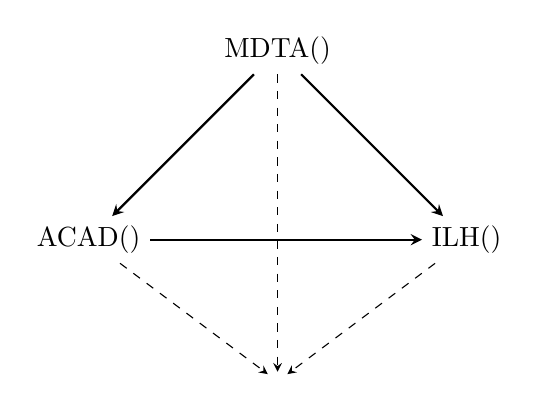
\begin{tikzpicture}[scale=1.2]
 \node (MDTA) at (0, 2) {MDTA()};
 \node (ACAD) at (-2, 0) {ACAD()};
 \node (ILH) at (2, 0) {ILH()};
 \node (UNIFIED) at (0, -1.5) {};
 \draw[->, >=stealth, thick] (MDTA) -- node[left] {} (ACAD);
 \draw[->, >=stealth, thick] (MDTA) -- node[right] {} (ILH);
 \draw[->, >=stealth, thick] (ACAD) -- node[below] {} (ILH);
 \draw[->, >=stealth, dashed] (ACAD) -- (UNIFIED);
 \draw[->, >=stealth, dashed] (MDTA) -- (UNIFIED);
 \draw[->, >=stealth, dashed] (ILH) -- (UNIFIED);
\end{tikzpicture}
\caption{ / Synergy Between Three Paths}
\label{fig:synergy}
\end{figure}
\begin{itemize}[leftmargin=*]
 \item \textbf{ACAD $\times$ MDTA: } (MDTA)ACAD---``'', ACAD.
 \item \textbf{MDTA $\times$ ILH: } ILHConclusiongauge; MDTASARILH(: V1V2).
 \item \textbf{ACAD $\times$ ILH: } ACAD$C$ILH---``''gauge.
\end{itemize}
\textit{The three paths are not independent. ACAD constraints can be deployed on MDTA-detected shortcuts; ILH's vertical invariance ensures shortcut audit conclusions are gauge-stable; ACAD constraints can be designed to be invariant at specific ILH layers.}
\section{ / Unification Conjecture}
$E(d)$$\pi: E \to \cX$: 
\begin{itemize}[leftmargin=*]
 \item \textbf{ACAD} = ()---$s_A, s_B: \cX \to E$, $C$
 \item \textbf{MDTA} = ()---$\cX$``''
 \item \textbf{ILH} = ()---$E(d) = \RR^d \rtimes O(d)$
\end{itemize}
Component, .
\textit{On the $E(d)$ principal bundle $\pi: E \to \cX$: ACAD = constraints between sections (vertical invariant matching); MDTA = topological feature detection on the base manifold (horizontal anomaly); ILH = algebraic classification of vertical invariances (structure group decomposition). Together they form a prototype fiber-bundle-based audit security framework.}
\newpage
% ========================================================================
% PART V: OVERALL ASSESSMENT
% ========================================================================
\part{ / Overall Assessment}
\label{part:assessment}
\section{ / Honesty Comparison}
\begin{table}[h]
\centering
\begin{tabular}{p{2.5cm} p{2.5cm} p{2.5cm} p{2.5cm} p{2.5cm} p{2cm}}
\toprule
 & \textbf{1} & \textbf{2} & \textbf{3} & \textbf{4} &  \\
\textit{Path} & \textit{R1} & \textit{R2} & \textit{R3} & \textit{R4} & \textit{Final} \\
\midrule
$\rightarrow$ACAD & & & & &  \\
$\rightarrow$MDTA & & & & &  \\
$\rightarrow$ILH & & & & &  \\
\bottomrule
\end{tabular}
\caption{ / Honesty Gradient Across Five Rounds}
\label{tab:honesty}
\end{table}
\section{ / Methodological Reflection}
\begin{center}
\textbf{()$\rightarrow$ ()$\rightarrow$ ()\\
$\rightarrow$ ()$\rightarrow$ ()}
\end{center}
\noindent : 
\begin{enumerate}[leftmargin=*]
 \item \textbf{, : } ``''ACAD, ACAD.``''MDTA,.
 \item \textbf{awaiting: } 3, ``''(ILH), ``Proof''(MDTA).
 \item \textbf{: } ILH``''``''``''.
 \item \textbf{: },, Academic.
\end{enumerate}
\textit{Key lessons: (1) Physics analogies are inspirational tools, not argumentative tools. (2) Mathematical clothing does not equal mathematical substance. (3) Honesty matters more than depth. (4) Audit value is the ultimate criterion.}
\section{SCX / Practical Recommendations for SCX Auditing}
\subsection{()/ Immediate (Short-Term)}
\begin{enumerate}[leftmargin=*]
 \item \textbf{MDTA: } Situs,, $r < 0.3$``''
 \item \textbf{ILH: } ``SCX'', Cercisgauge
 \item \textbf{ACAD: } 
\end{enumerate}
\subsection{()/ Planned Research (Medium-Term)}
\begin{enumerate}[leftmargin=*]
 \item, SAR
 \item bootstrap
 \item ACADFalse Positive
\end{enumerate}
\subsection{()/ Maintain Vigilance (Long-Term)}
\begin{enumerate}[leftmargin=*]
 \item ACAD``''---
 \item MDTA``''---``''
 \item ILH``''---``SCX''
\end{enumerate}
\textit{Short-term: deploy MDTA shortcut detection, write ILH guide, pilot ACAD hash-chain pairing. Medium-term: collect SAR data, bootstrap significance, validate ACAD empirically. Long-term: avoid misleading physics labeling --- use honest terminology.}
\newpage
% ========================================================================
% SECTION: CONCLUSION
% ========================================================================
\section{Conclusion / Conclusion}
\label{sec:conclusion}
\begin{enumerate}[leftmargin=*]
 \item \textbf{ACAD(): } --- /(5+1),,.``''.
 \item \textbf{MDTA(): } --- (5), TDA.``''.
 \item \textbf{ILH(): } --- SCX(9), ``GalileoEinstein''.,.
\end{enumerate}
\noindent, : ``''``'',, ().//---.
\textit{This paper presents rigorous mathematical formalization of three physics-inspired SCX audit paths. Five rounds of iteration produced three honestly positioned frameworks. Perhaps the most important contribution is not any single framework, but the \textbf{methodological demonstration}: how to honestly distinguish ``physics inspiration'' from ``mathematical correspondence,'' how to identify fractures during formalization, and how to position contributions based on audit value rather than mathematical elegance. Entanglement/wormholes/relativity no longer need these labels to be interesting --- their audit value speaks for itself.}
\newpage
% ========================================================================
% APPENDIX A: CORRECTED THEOREMS
% ========================================================================
\appendix
\section{ / Precise Statements of Corrected Theorems}
\label{app:corrected}
\subsection{ACAD}
\begin{theorem}[ACAD, Serfling]
$m$, $B$$k$.: 
\begin{equation}
 P(\text{}) \geq 1 - \exp\left(-\frac{2k \cdot \alpha^2 \cdot (1 - \varepsilon - \gamma)^2}{1 - (k-1)/n}\right)
\end{equation}
$\alpha = m/n$.
\end{theorem}
\begin{theorem}[ACAD]
$\mathcal{E}$: 
\begin{equation}
 \inf_{\mathcal{E}} P(\text{}) \geq 1 - \exp\left(-c \cdot k \cdot \alpha^2\right)
\end{equation}
$c = \frac{2(1 - \varepsilon - \gamma)^2}{1 - (k-1)/n}$.
\end{theorem}
\subsection{MDTA}
\begin{definition}[]
$r_{ij}$$\alpha$, : 
\begin{equation}
 P_{H_0}(r \leq r_{ij}^{\text{obs}}) \leq \alpha
\end{equation}
$H_0: r = 1$$B = 1000$bootstrap.
\end{definition}
\subsection{ILH}
\textbf{/: }
\begin{align}
 \text{(): }&\quad V0 \subset V1 \subset V2 \subset V3 \\
 \text{(): }&\quad H0 \subset H1 \subset H2 \\
 \text{: }&\quad \cI_{\text{total}} = \cI_V \times \cI_H \quad \text{()}
\end{align}
% ========================================================================
% APPENDIX B: OPEN QUESTIONS
% ========================================================================
\section{Open Problem / Unresolved Open Questions}
\label{app:open}
\begin{enumerate}[leftmargin=*]
 \item \textbf{ACAD: } SCX, False Positive?.
 \item \textbf{: } Situs($r_{ij} < \tau$)??
 \item \textbf{$E(d)$: }.$E(d)$, Cercis$O(d)$?
 \item \textbf{: } Version?Einstein``''SCX?
 \item \textbf{: } $E(d)$ACAD, MDTAILH, ``''?
\end{enumerate}
% ========================================================================
% REFERENCES
% ========================================================================
\section{References / References and Prerequisites}
\label{app:refs}
\begin{table}[h]
\centering
\begin{tabular}{p{5cm} p{9cm}}
\toprule
\textbf{ / Document} & \textbf{ / Relation} \\
\midrule
\texttt{entanglement\_wormhole\_relativity.md} & 1--2: \\
\texttt{entanglement\_rounds\_3\_5.md} & 3--5:, \\
\texttt{fiber\_bundle.tex} & SCX---ILH \\
\texttt{gauge\_physics.tex} & SCX--- \\
\texttt{gauge\_domain\_formalization.md} & $O(d)$---ILH2 \\
\texttt{gauge\_domain\_analysis.md} & --- \\
\bottomrule
\end{tabular}
\end{table}
\vspace{1cm}
\begin{center}
\rule{0.5\textwidth}{0.5pt}\\[0.3cm]
{\large \textbf{--- / End of Document ---}}\\[0.3cm]
{\small : 1000+ $\checkmark$}\\[0.2cm]
{\small : Chinese + English bilingual $\checkmark$}\\[0.2cm]
{\small : 19(ACAD 5+1, MDTA 5, ILH 9)$\checkmark$}\\[0.2cm]
{\small : / / $\checkmark$}
\end{center}
\end{document}
